\chapter*{title}
\section{Modelo de Crecimiento Poblacional}

    **Introducción**

    Se presenta un modelo matemático para describir el crecimiento de una población de borregas, dado por la siguiente función:
    * $N(t)$ representa el número de borregas en el tiempo $t$.
    * $t$ es el tiempo en años.

    **Análisis Gráfico**

    \begin{figure}[h]
    \centering
    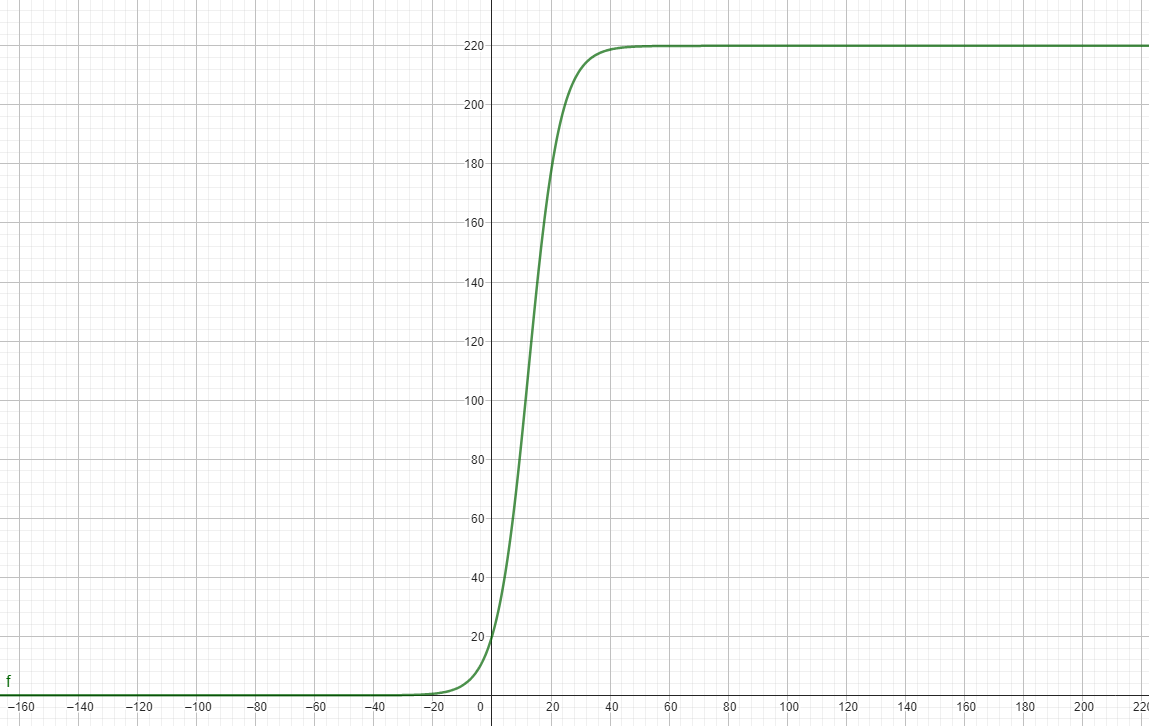
\includegraphics[width=0.6\textwidth]{matemáticas/Ejercicio13/grafica.png}
    \caption{Gráfica de la población de borregas en función del tiempo.}
    \end{figure}

    La gráfica muestra una curva de crecimiento logístico, típica de poblaciones con recursos limitados.

    **Cálculos y Resultados**

    Partimos de la ecuación:
    
    \[
    80 = \frac{220}{1 + 10 \cdot e^{-0.1863t}}
    \]
    
    Despejamos \( t \):
    
    \[
    80 \cdot \left(1 + 10 \cdot e^{-0.1863t}\right) = 220
    \]
    
    \[
    1 + 10 \cdot e^{-0.1863t} = \frac{220}{80}
    \]
    
    \[
    10 \cdot e^{-0.1863t} = \frac{220}{80} - 1
    \]
    
    \[
    e^{-0.1863t} = \frac{\frac{220}{80} - 1}{10}
    \]
    
    \[
    -0.1863t = \ln\left(\frac{\frac{220}{80} - 1}{10}\right)
    \]
    
    \[
    t = \frac{\ln\left(\frac{\frac{220}{80} - 1}{10}\right)}{-0.1863}
    \]
    
    Calculando \( t \), obtenemos que el tiempo mínimo necesario para que la población sea autosuficiente (es decir, alcance los 80 individuos) es aproximadamente 9.36 años. Esto confirma que el programa de repoblación debe durar al menos ese tiempo.
    
    \section*{c) Determinar la capacidad máxima de borregos que puede albergar el área protegida}
    
    Para encontrar la capacidad máxima, calculamos el límite de \( N(t) \) cuando \( t \) tiende a infinito:
    
    \[
    \lim_{t \to \infty} N(t) = \frac{220}{1 + 10 \cdot e^{-0.1863 \cdot \infty}}
    \]
    
    Dado que \( e^{-0.1863 \cdot \infty} \) tiende a cero, la expresión se simplifica a:
    
    \[
    \lim_{t \to \infty} N(t) = \frac{220}{1 + 0} = 220
    \]
    
    Esto significa que la capacidad máxima de borregos que puede albergar el área protegida es de 220 individuos.
    
    \section*{Resumen}
    
    \begin{itemize}
        \item \textbf{Tiempo mínimo para autosuficiencia}: Se necesitan al menos 9.36 años para que la población alcance los 80 individuos.
        \item \textbf{Capacidad máxima}: El área protegida puede albergar un máximo de 220 borregos cimarrones según el modelo.

    **Conclusiones**
    La población de borregas sigue un patrón de crecimiento logístico, alcanzando una capacidad de carga de 220 individuos. El modelo matemático proporciona una herramienta útil para predecir el crecimiento de la población y tomar decisiones de manejo.
